\chapter{新高出力モータドライバ}

\section{要求機能}
ロボコンで使用するバッテリーは,最大電圧14.8V,最大電流178Aで,モータは最大電流130Aである.
このことから,ITOLAB MOTORDRIVERでバッテリー,モータの性能を最大まで発揮できていない
ことが分かる.
これを考慮した上で,
先に述べた不具合箇所を修正,改良した高出力モータドライバを製作した.
\begin{itemize}
\item 大電流が流れるパターン幅の拡張,GNDのベタ化
\item FETヒートシンク,回生ダイオードの標準搭載
\item FET用温度センサの取り付け
\item モータに流れる電流を確認するための電流センサの取り付け
\item エラー,通信を確認するための汎用LEDの取り付け
\item 制御用マイコンのリセットスイッチ,実験などに使用できる汎用スイッチの搭載
\item ノイズの影響を受けやすいRS232通信から,影響の受けにくい作動伝送を用いた
RS485通信への変更
\end{itemize}


\section{構成}
新高出力モータードライバのシステムブロック図を図\ref{fig:shisutemu}に示す.
また,新モータドライバの仕様書を表\ref{tab:shinshiyou}に示す.付録CにRXマイコンと
各部品との接続を示した.
\begin{figure}[H]
  \begin{center}
    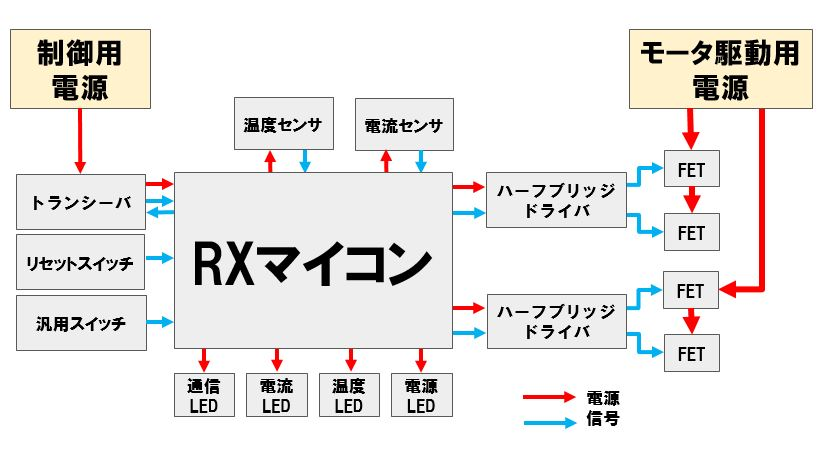
\includegraphics[width=150mm]{shisutemu}
    \end{center}
  \caption{システムブロック図}
 \label{fig:shisutemu}
\end{figure}
\begin{table}[htb]
\centering
\caption{新モータドライバの仕様書}
\begin{tabular}{|c|c|} \hline
使用マイコン&RX220マイコン\\ \hline
シリアル通信&RS485\\ \hline
FET&$V_{DS}$  40V\\
   &$I_D$  80A  \\ \hline
温度センサ&動作温度 -40~125℃ \\
&動作電圧 3.1~5.5V \\ \hline
電流センサ&動作温度 -40~150℃\\
&作動電圧 3.3~5.5V \\
&検出電流 0~100A \\ \hline
最大定格電圧&40V\\ \hline
最大定格電流&80A\\ \hline
\end{tabular}
\label{tab:shinshiyou}
\end{table}

\section{回路図・アートワーク図}
ロボコン用高出力モータードライバの回路図,アートワーク図をそれぞれ図\ref{fig:kairozu}
,図\ref{fig:a-towa-ku}に示す.また,基板の3Dビューアを図\ref{fig:3Dbyu-a}に示す.
回路図,アートワークの作成は,回路図とアートワークが連動しているKiCadを用いた.
回路図は,ITOLAB MOTORDRIVERの回路図を作成した後に,新たな部品を接続した.

アートワークは,大電流の流れる可能性のあるパターン幅を,1.0mmから5.0mmに変更した.
パターン幅と電流許容量は比例しているので,電流の許容量は5倍になる.
また,裏面はGNDのベタ化を行った.
\begin{figure}[H]
\begin{center}
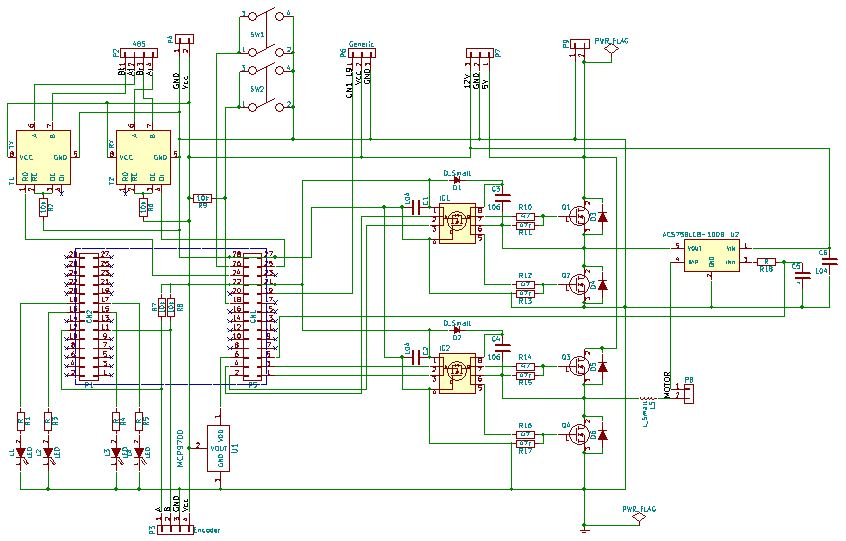
\includegraphics[width=150mm]{kairozu}
\end{center}
\caption{回路図}
\label{fig:kairozu}
\end{figure}
\begin{figure}[H]
\begin{center}
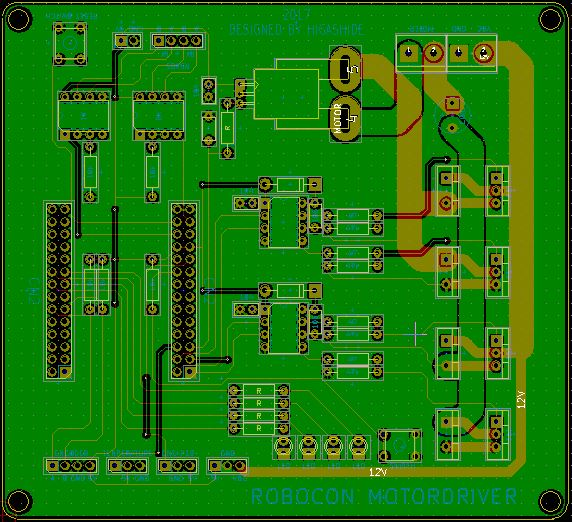
\includegraphics[width=150mm]{a-towa-ku}
\end{center}
\caption{アートワーク図}
\label{fig:a-towa-ku}
\end{figure}
\begin{figure}[H]
\begin{center}
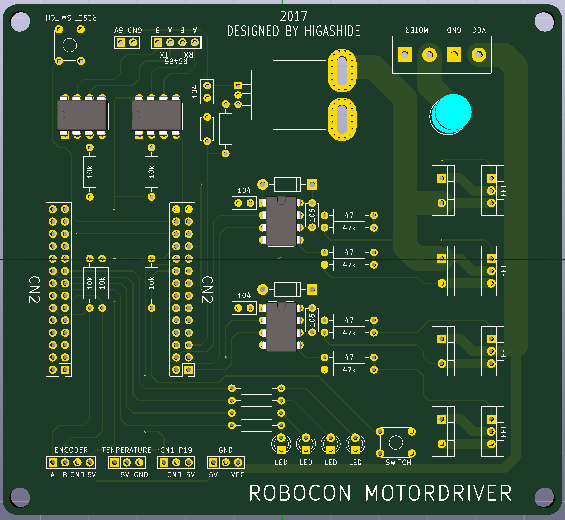
\includegraphics[width=150mm]{3Dbyu-a}
\end{center}
\caption{3Dビューア}
\label{fig:3Dbyu-a}
\end{figure}

\section{完成品}
ロボコン用高出力モータドライバの完成品を図\ref{fig:kansei}に,組み付けたものを図\ref{fig:kankumi}に示す.
基板の製作は,Fusion PCBに依頼した.
\begin{figure}[H]
\begin{center}
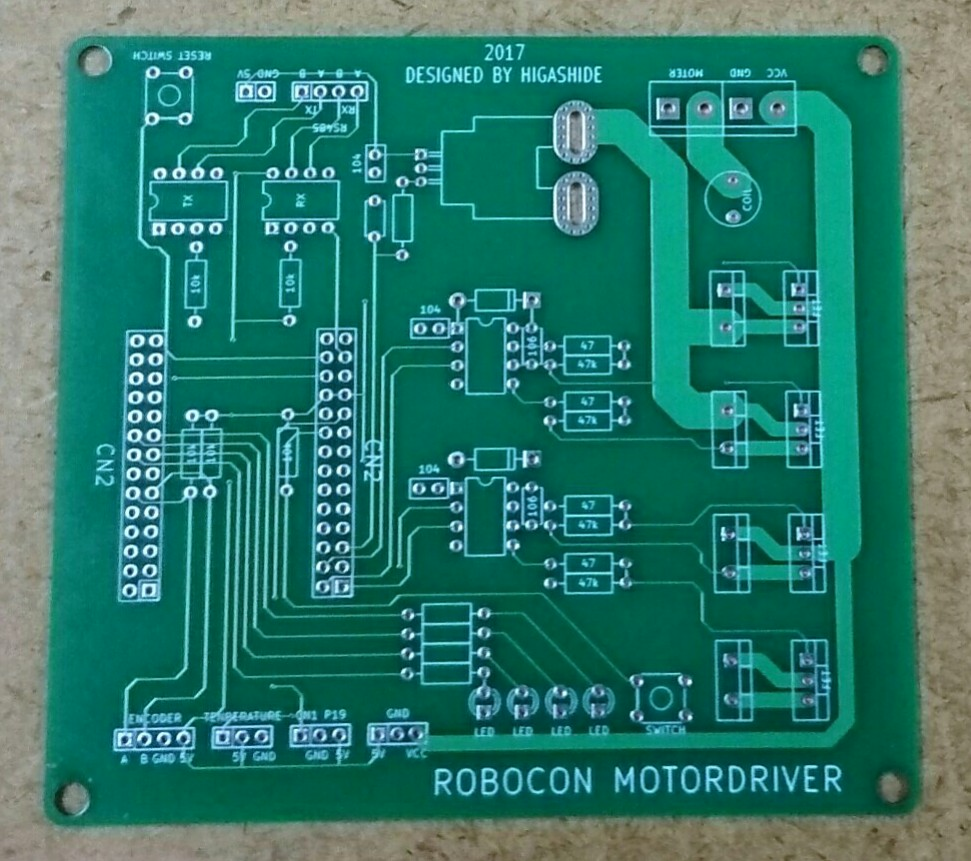
\includegraphics[width=150mm]{kansei}
\end{center}
\caption{完成品}
\label{fig:kansei}
\end{figure}
\begin{figure}[H]
\begin{center}
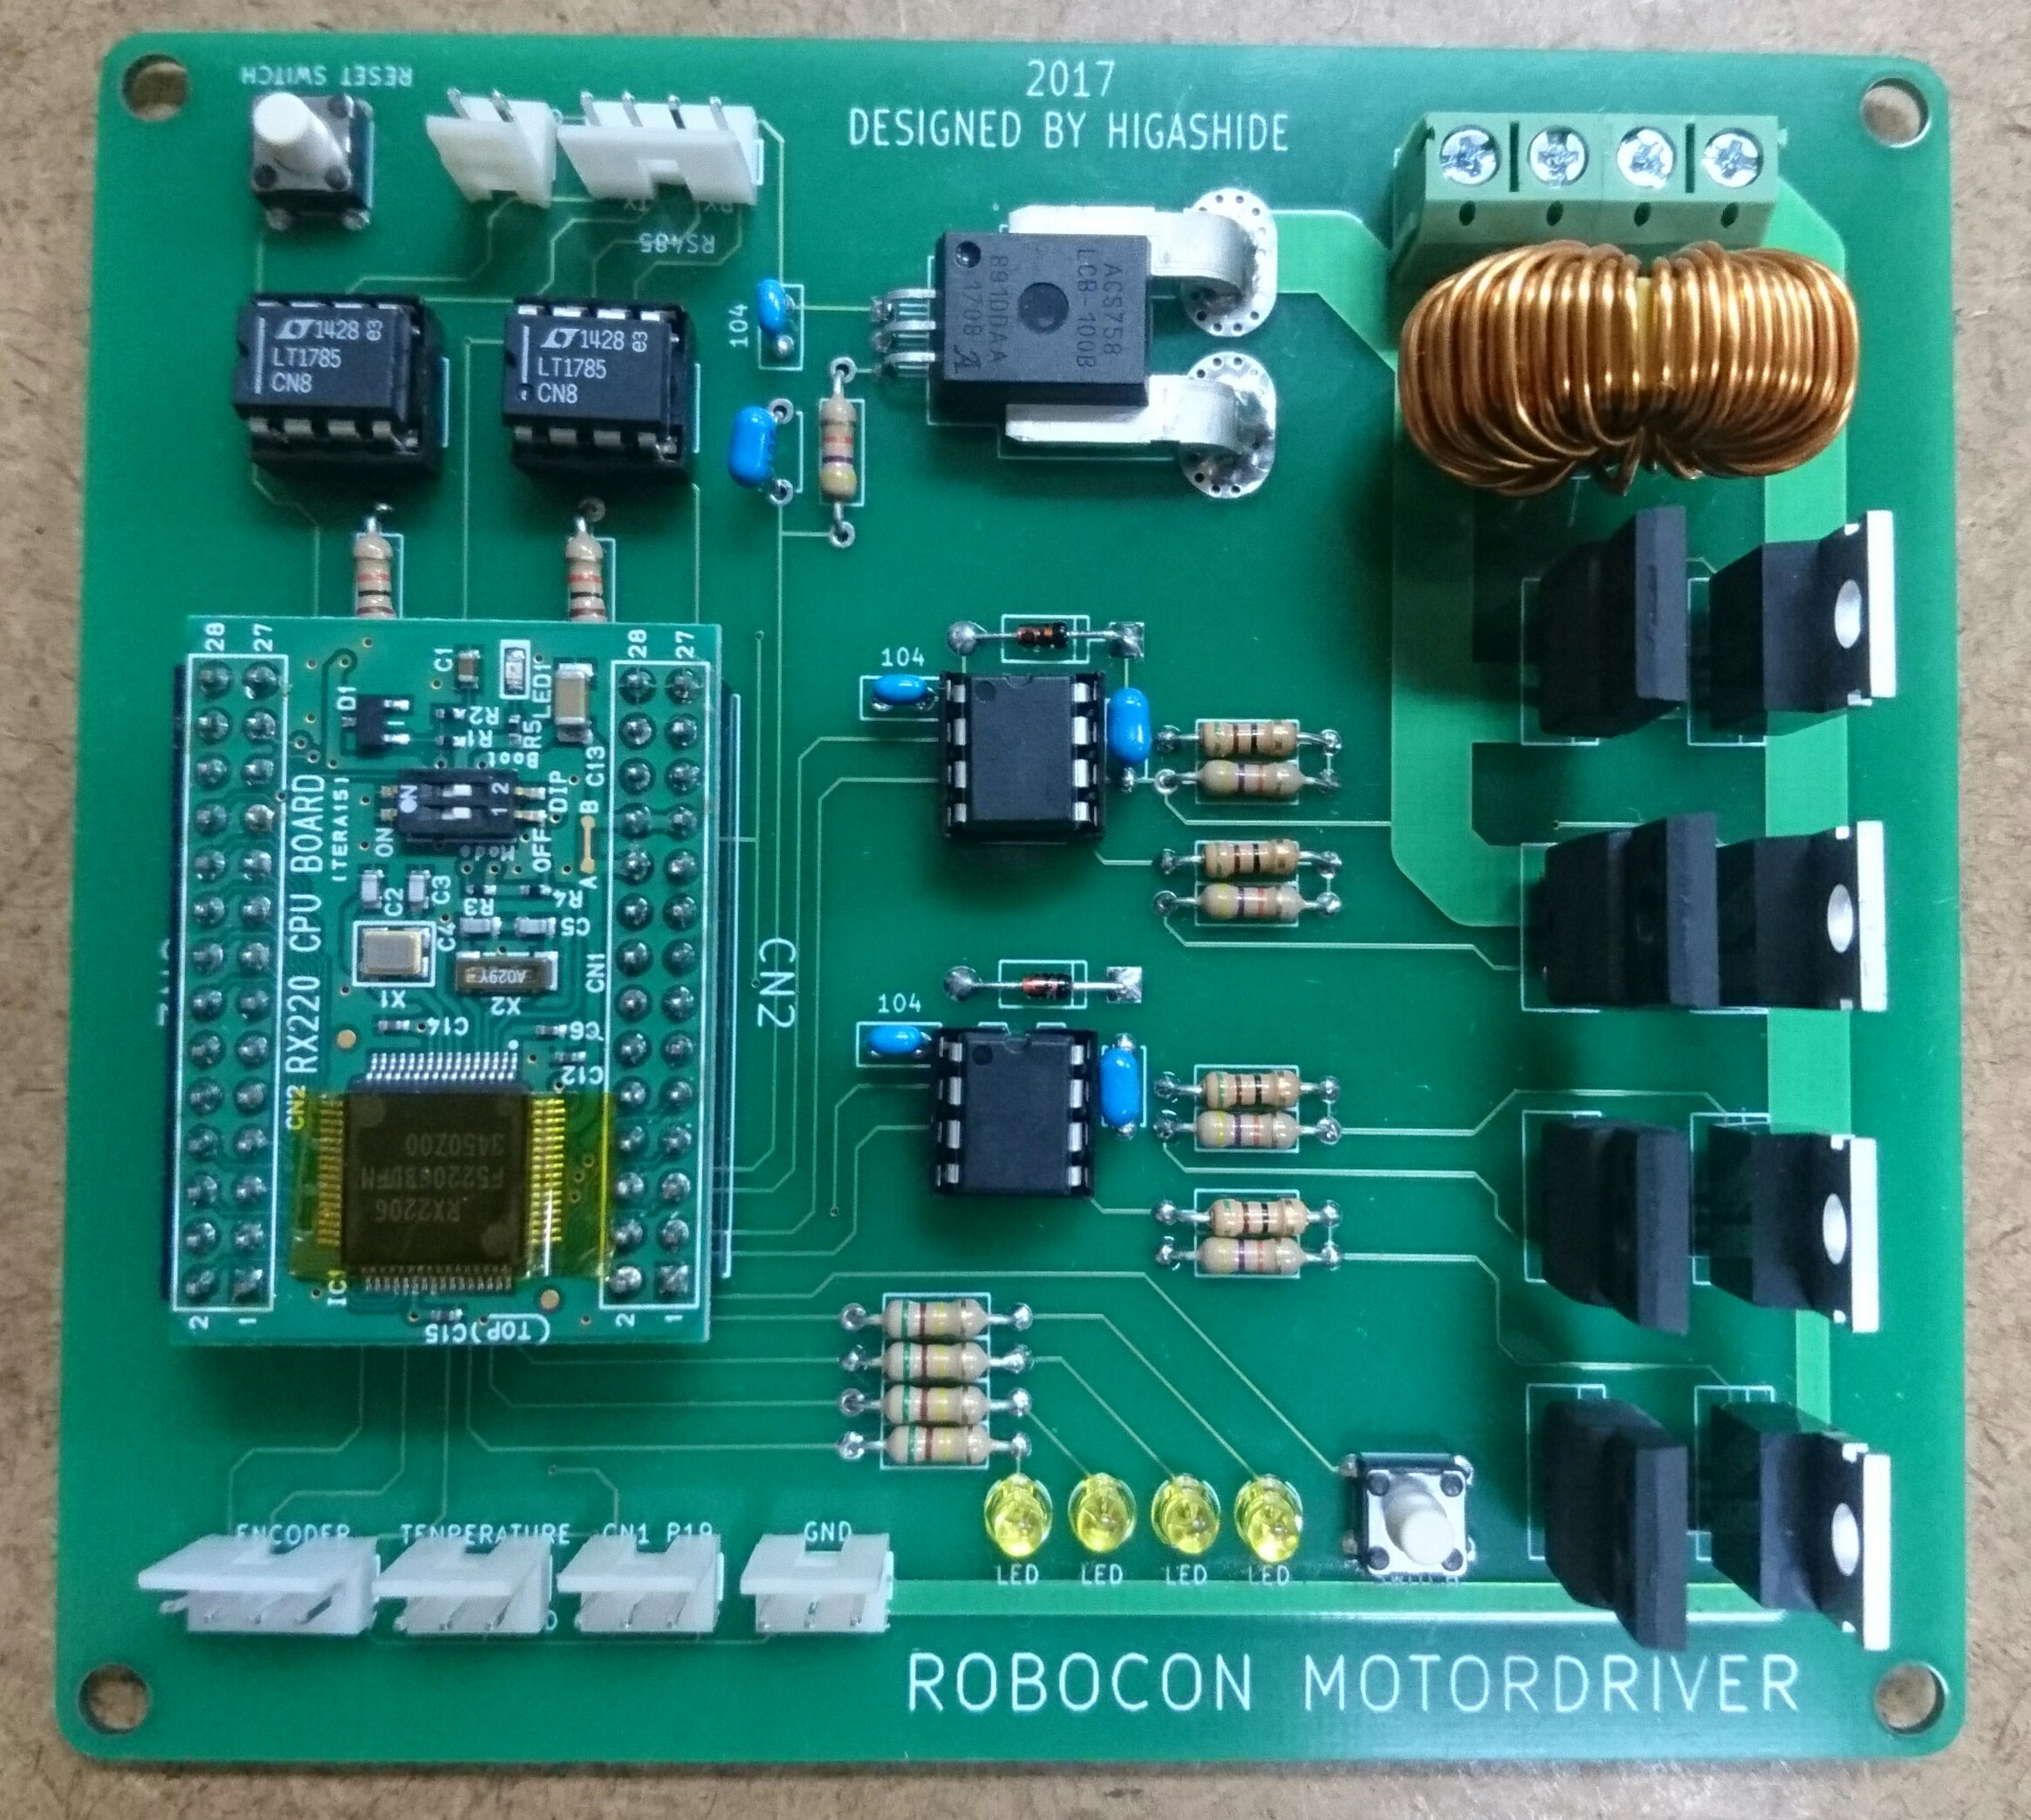
\includegraphics[width=150mm]{kankumi}
\end{center}
\caption{組み付け後}
\label{fig:kankumi}
\end{figure}

\section{実機の動作実験}
動作の確認として以下の実験を行った.
\begin{itemize}
\item LEDが点灯するか
\item 汎用スイッチが動作するか
\item リセットスイッチでRXマイコンのリセットが可能か
\item RXマイコンからPWM信号の出力が可能か
\end{itemize}

\section{実験結果}
実験の結果,以下のようになった.
\begin{itemize}
\item 図\ref{fig:jikken}のように,LEDの点灯を確認
\item 汎用スイッチ動作を確認
\item リセットスイッチでリセット確認
\item PWM信号の出力により,モータが回転することを確認
\end{itemize}
\begin{figure}[H]
\begin{center}
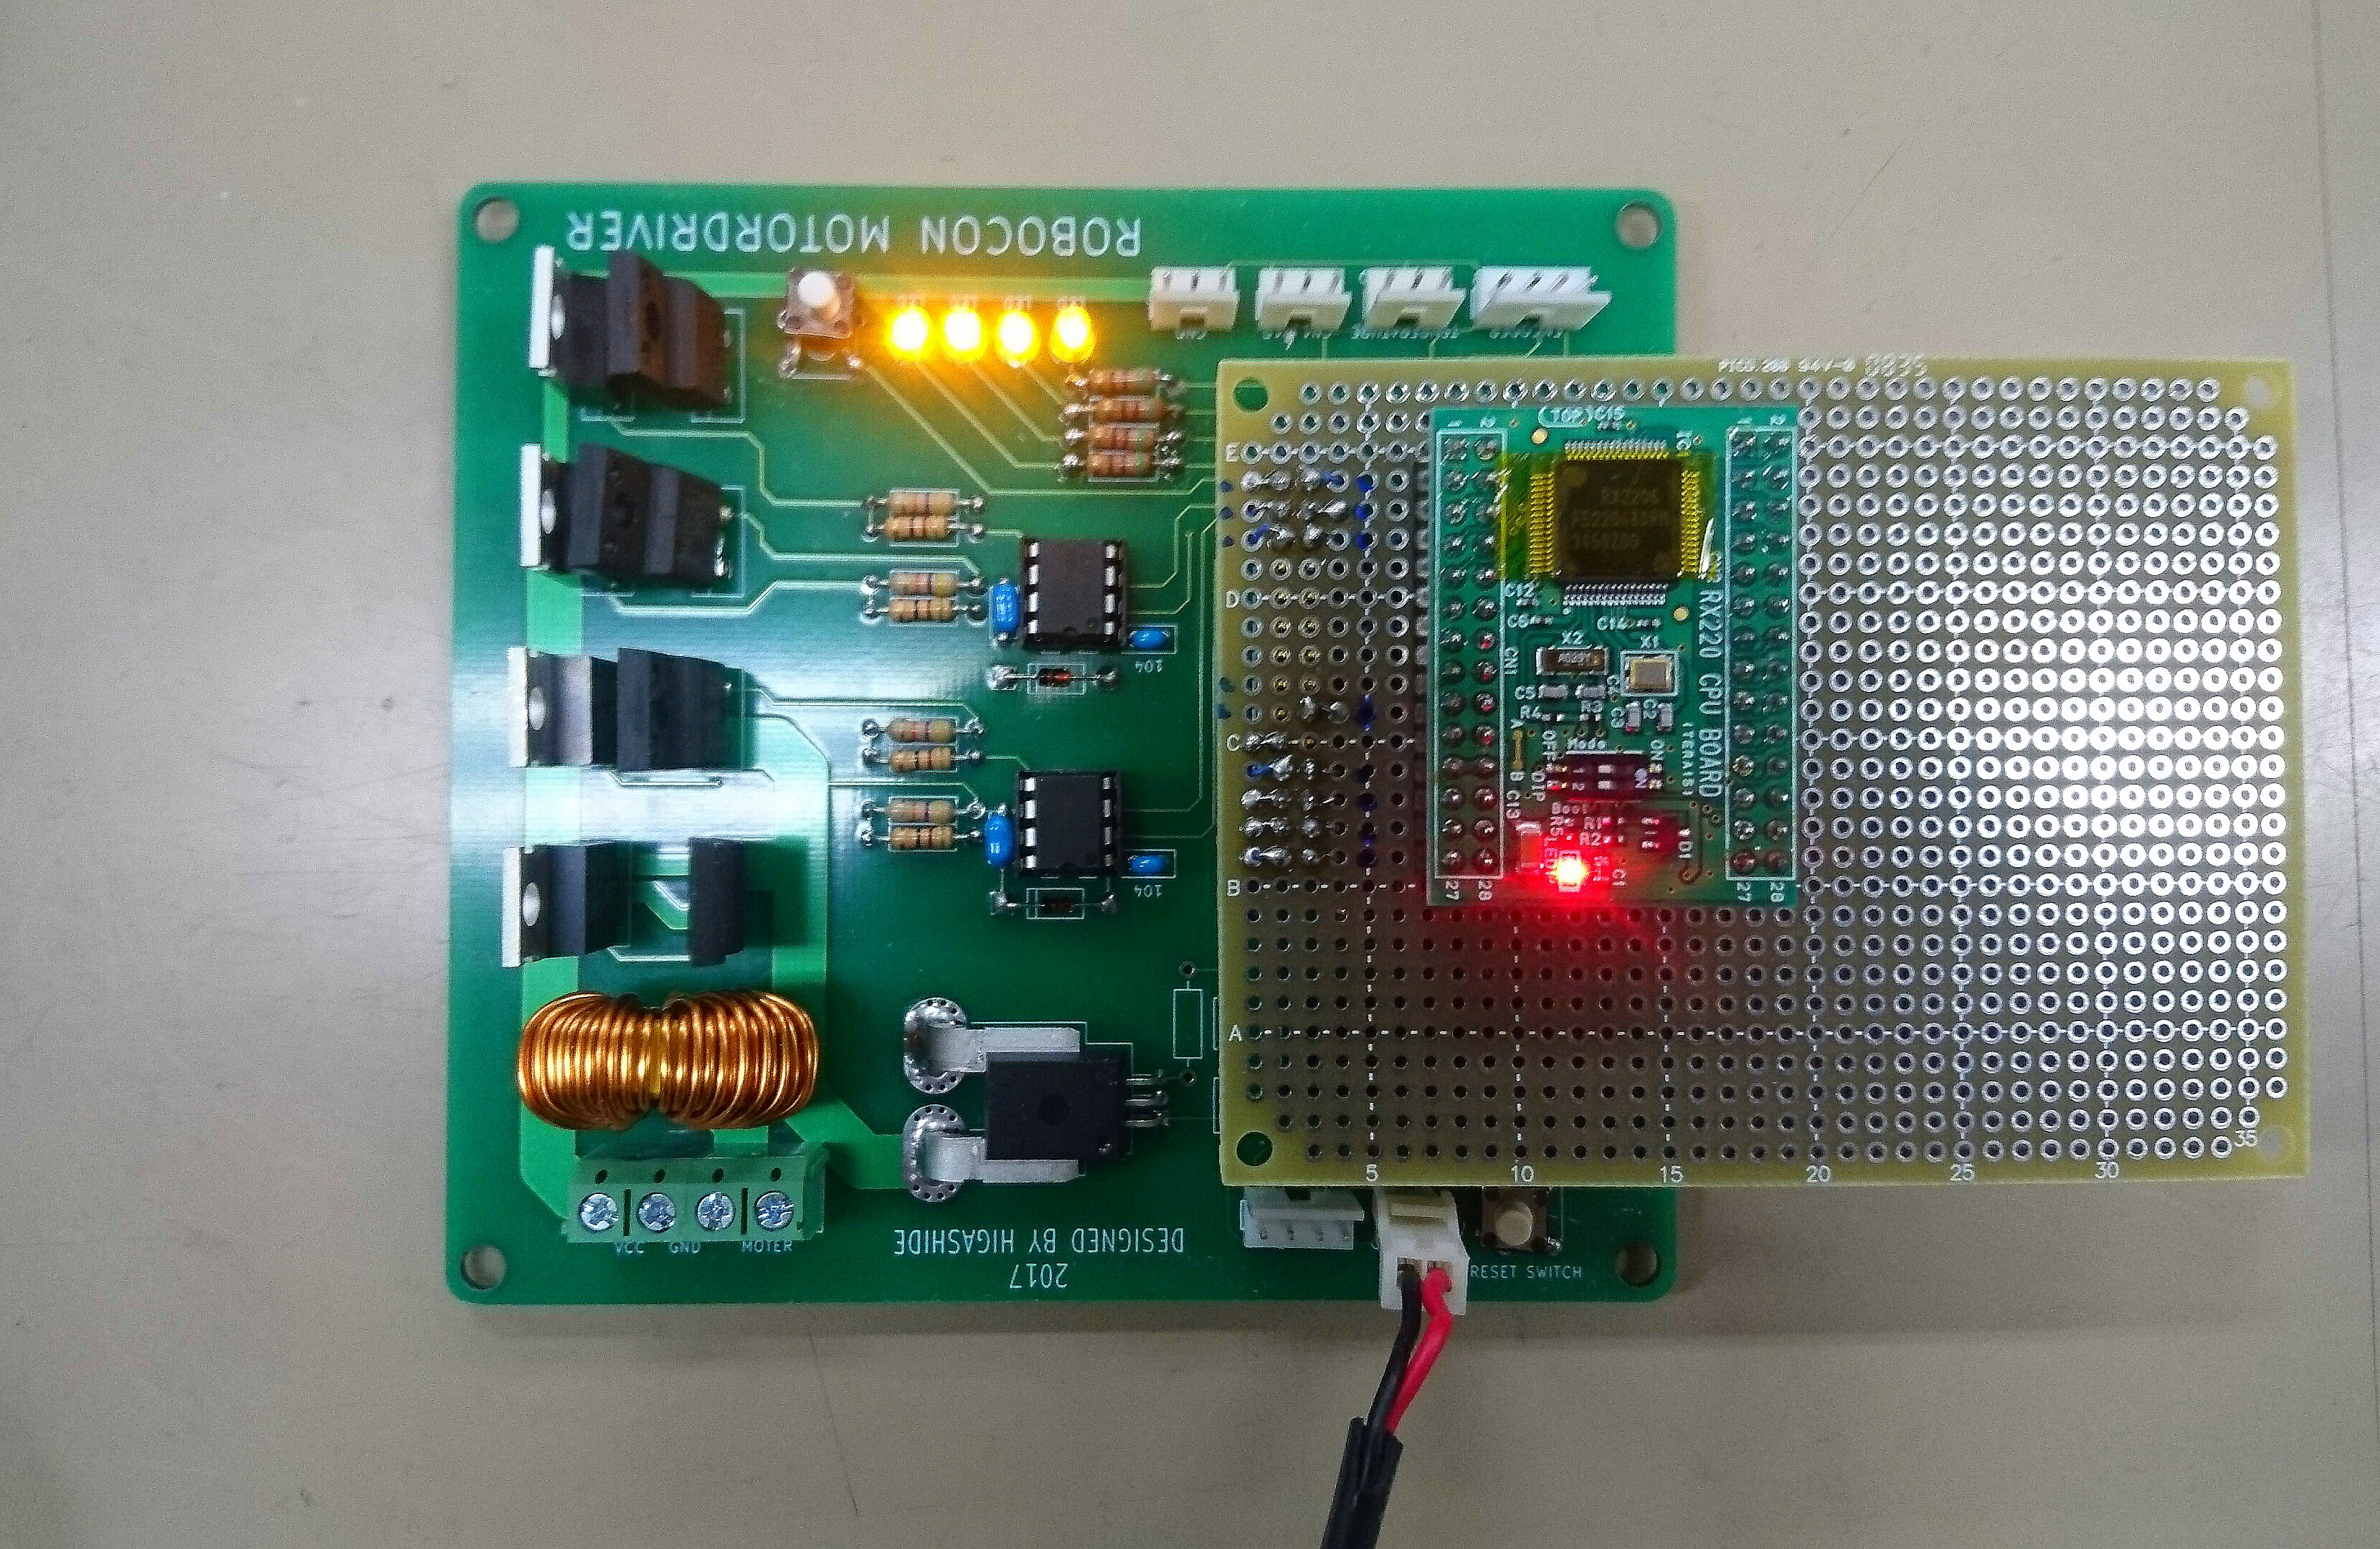
\includegraphics[width=140mm]{jikken}
\end{center}
\caption{LEDの点灯している高出力モータドライバ}
\label{fig:jikken}
\end{figure}

\section{考察}
以上の結果から,配線の間違いはないことが分かる.
また,モータが回転したことから,RXマイコンのPWM信号でハーフブリッジドライバ,FETが問題
なく機能していることが分かる.
